\documentclass[10pt]{article}

\usepackage{geometry}
\geometry{margin=1in}

\usepackage{tikz}
\usetikzlibrary{arrows.meta,positioning,calc} 

\usepackage{hyperref}
\usepackage{graphicx}
\usepackage{listings}
\usepackage{amsmath}

\title{Drop-In JTAG: Lightweight HDL-Based Debug and Data Extraction Interface \\ Version 1.0.0}
\author{James E. Stine}
\date{\today}

\begin{document}

\maketitle

\section{Introduction}

Debugging digital hardware designs often requires visibility into internal signals that are otherwise inaccessible once a design is synthesized onto an FPGA or ASIC. Traditional debugging approaches such as logic analyzers or integrated logic analyzers (ILA) require either dedicated hardware resources or significant integration effort.

This document describes \textit{Drop-In JTAG}, a lightweight HDL-based instrumentation technique that allows internal signals to be extracted through a JTAG interface with minimal integration effort.

The project repository is available at:

\begin{center}
\url{https://github.com/stineje/Drop-In-JTAG}
\end{center}

The goal of Drop-In JTAG is to provide a reusable mechanism that allows designers to easily capture and shift out internal signals without requiring specialized debug IP.

\section{Concept Overview}

Drop-In JTAG borrows concepts from the IEEE 1149.1 boundary scan architecture but implements a simplified mechanism entirely in synthesizable HDL~\cite{ieee1149}.

Rather than relying on physical boundary scan cells integrated into IO pads, Drop-In JTAG inserts HDL-based scan cells directly into the design hierarchy. These cells allow selected signals to be captured and shifted out through the JTAG interface.

The approach provides:

\begin{itemize}
\item Minimal design modification
\item Reusable debug infrastructure
\item Compatibility with standard JTAG interfaces
\item Applicability to both FPGA and ASIC environments
\end{itemize}

\section{Relation to Boundary Scan}

IEEE 1149.1 boundary scan places scan cells at the periphery of a chip to allow testing of interconnect between devices. Each IO pin contains a boundary scan cell that can capture and shift values through a scan chain.

Drop-In JTAG uses a conceptually similar scan-chain architecture but differs in several important ways:

\begin{itemize}
\item Cells are implemented in HDL rather than dedicated silicon boundary cells.
\item Signals monitored are internal design signals rather than IO pins.
\item The structure is intended primarily for debugging and observability rather than manufacturing test.
\end{itemize}

Thus, while the mechanism resembles boundary scan, it should be viewed as a \textit{boundary-scan-inspired instrumentation technique} rather than a strict IEEE 1149.1 implementation.

\section{Architecture}

The Drop-In JTAG architecture consists of three primary components:

\begin{itemize}
\item JTAG interface logic
\item Boundary-scan style register cells
\item Scan chain connecting the cells
\end{itemize}

Selected internal signals are connected to scan cells. These cells capture the signal values and shift them out through the JTAG scan chain.

\subsection{Scan Cell Operation}

Each scan cell contains:

\begin{itemize}
\item Capture register
\item Shift register
\item Mode control
\end{itemize}

During operation:

\begin{itemize}
\item \textbf{Capture}: internal signal values are sampled
\item \textbf{Shift}: data is shifted through the scan chain
\item \textbf{Update}: optional update of driven signals
\end{itemize}

\section{Boundary Scan and Scan-Chain Operation}

The scan cells are instantiated in the top-level design. For example:
\begin{lstlisting}[language=Verilog, basicstyle=\ttfamily\small]
bsr #(.WIDTH(32)) InstrF_bsr (
    .clk(bsr_clk),
    .update_dr(bsr_update),
    .shift_dr(bsr_shift),
    .mode(bsr_mode),
    .tdi(bsr_chain[1]),
    .tdo(bsr_chain[2]),
    .parallel_in(InstrF),
    .parallel_out(InstrF_internal)
);
\end{lstlisting}
This cell allows the internal signal \texttt{InstrF} to be captured and shifted through the JTAG scan chain.

The Drop-In JTAG infrastructure is conceptually derived from the scan-chain mechanisms used in IEEE 1149.1 boundary scan. In a traditional boundary scan architecture, each digital IO pin of an integrated circuit contains a boundary scan cell. These cells are connected together to form a serial shift register that spans the periphery of the device. The scan chain is accessed through the JTAG Test Access Port (TAP), which consists of the signals TCK, TMS, TDI, and TDO. During boundary scan operation, the TAP controller places the device into states that allow data to be captured into the scan cells, shifted serially through the chain, and optionally updated back into the device. Because the scan cells are connected sequentially, the state of many signals can be captured and shifted out through a single serial data path.

The Drop-In JTAG approach follows a similar conceptual structure but implements the scan cells entirely within synthesizable HDL rather than as dedicated boundary scan hardware within IO pads. Each scan cell captures the value of a selected internal signal and inserts that value into a serial scan chain. The cells are connected through signals such as \texttt{tdi} and \texttt{tdo}, forming a chain that propagates serial data through the design. When the shift operation is active, data is shifted from one cell to the next in synchronization with the JTAG clock. As the scan chain shifts, captured values propagate toward the end of the chain and eventually appear on the JTAG data output signal.

Because the cells are connected sequentially, the scan chain behaves as a long shift register embedded within the HDL design. Each cell receives serial input data from the previous cell and forwards serial output data to the next cell in the chain. During capture operations, each cell stores the current value of the monitored signal. During shift operations, these stored values move through the chain one bit position at a time. This serialized propagation of internal signal values allows a large amount of state information to be extracted using only the JTAG serial interface.

In Drop-In JTAG, the scan cells are typically instantiated in the top-level HDL module and connected together through a chain of intermediate signals such as \texttt{bsr\_chain}. Each element of the chain connects the \texttt{tdo} output of one cell to the \texttt{tdi} input of the next cell. The first cell in the chain receives data from the external JTAG data input, while the final cell drives the JTAG data output. This structure forms a continuous serial path that allows captured signal values to propagate through the design and ultimately be retrieved through the JTAG interface.

Although this mechanism resembles boundary scan in its use of capture and shift operations, its purpose differs from conventional boundary scan testing. Rather than focusing on board-level interconnect verification, the Drop-In JTAG infrastructure provides observability into internal design signals. The scan-chain mechanism therefore functions primarily as a debugging and instrumentation interface that enables internal state extraction without requiring dedicated debug IP cores or specialized hardware instrumentation.

Figure~\ref{fig:scan_chain} illustrates the conceptual structure of the Drop-In JTAG scan chain implemented in the HDL design. Each scan cell forms part of a serial chain in which data propagates from the JTAG data input (TDI) through a sequence of cells and eventually exits through the JTAG data output (TDO). Within each cell, the signal connected to the \texttt{parallel\_in} port represents the internal design signal that is observed by the instrumentation infrastructure. During a capture operation, the value of this signal is loaded into the cell and becomes part of the serial scan chain. The captured data can then be shifted through neighboring cells in synchronization with the JTAG clock until it appears at the scan-chain output.

The \texttt{parallel\_out} port allows the scan cell to optionally drive or forward a signal back into the surrounding design logic. This mechanism makes it possible to insert the scan cell into an existing signal path while maintaining functional connectivity of the original design. In this configuration, the scan cell acts as a lightweight boundary-scan-style register embedded within the HDL structure. By chaining multiple cells together using the \texttt{tdi} and \texttt{tdo} connections, internal signals from different parts of the design can be captured and serialized into a single scan path that is accessible through the JTAG interface.
\begin{figure}[h]
\centering
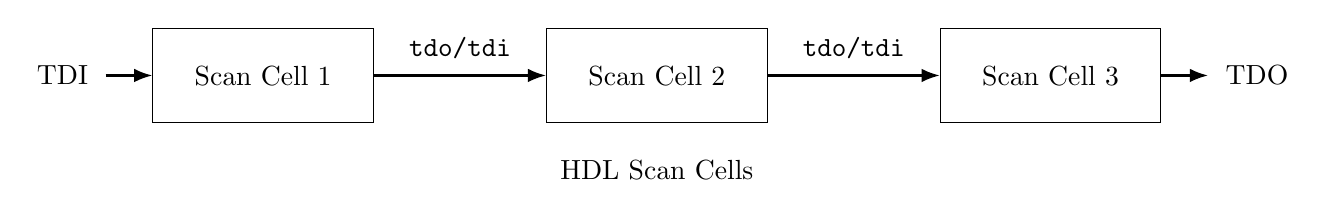
\begin{tikzpicture}[
    cell/.style={draw, rectangle, minimum width=2.8cm, minimum height=1.2cm, align=center},
    arrow/.style={-Latex, thick}
]

\node[cell] (c1) at (0,0) {Scan Cell 1};
\node[cell] (c2) at (5,0) {Scan Cell 2};
\node[cell] (c3) at (10,0) {Scan Cell 3};

% TDI side
\draw[arrow] (-2.0,0) -- (c1.west);
\node[anchor=east] at (-2.1,0) {TDI};

% Internal scan chain
\draw[arrow] (c1.east) -- (c2.west);
\node at (2.5,0.35) {\texttt{tdo/tdi}};

\draw[arrow] (c2.east) -- (c3.west);
\node at (7.5,0.35) {\texttt{tdo/tdi}};

% TDO side
\draw[arrow] (c3.east) -- (12.0,0);
\node[anchor=west] at (12.1,0) {TDO};

\node at (5,-1.2) {HDL Scan Cells};

\end{tikzpicture}
\caption{Conceptual diagram of the Drop-In JTAG scan chain. Each HDL scan cell captures an internal signal and shifts its contents serially through the chain using the JTAG interface.}
\label{fig:scan_chain}
\end{figure}

The implementation of the scan cell used in Drop-In JTAG is provided in the module \texttt{bsr.sv}, available in the repository at \url{https://github.com/stineje/Drop-In-JTAG/blob/main/JTAG-HDL/bsr.sv}. This module implements a boundary-scan-style register that supports capture, shift, and update operations under control of the JTAG interface signals. The module receives scan-chain control signals such as \texttt{shift\_dr} and \texttt{update\_dr} together with the scan clock and mode signals, and maintains the internal register state that participates in the serial scan chain. Listing~\ref{lst:bsr} shows the interface of the boundary-scan-style register used in the Drop-In JTAG infrastructure.

\begin{lstlisting}[language=Verilog, basicstyle=\ttfamily\footnotesize, caption={Excerpt from the Drop-In JTAG boundary-scan register implementation in \texttt{bsr.sv}.}, label={lst:bsr}]
module bsr #(parameter WIDTH=1)
(
    input  logic clk,
    input  logic update_dr,
    input  logic shift_dr,
    input  logic mode,
    input  logic tdi,
    output logic tdo,
    input  logic [WIDTH-1:0] parallel_in,
    output logic [WIDTH-1:0] parallel_out
);
\end{lstlisting}

During capture operations, the value presented on the \texttt{parallel\_in} port is stored in the internal register of the scan cell. When the JTAG interface enters the shift state, the stored value propagates serially through the scan chain using the \texttt{tdi} and \texttt{tdo} connections. The \texttt{parallel\_out} port allows the scan cell to optionally drive or forward a signal back into the surrounding design logic, enabling the scan cell to be inserted directly into an existing signal path while maintaining the functional behavior of the design. By chaining multiple \texttt{bsr} instances together, internal signals from across the design can be captured and serialized into a single scan path that is accessible through the JTAG interface.



\section{FPGA Demonstration}

The Drop-In JTAG infrastructure has been demonstrated on a Digilent Arty A7-100T FPGA platform.

The repository includes:

\begin{itemize}
\item HDL implementation
\item example FPGA design
\item scripts for interacting with the scan chain
\end{itemize}

\section{Python Interaction}

A Python script is included in the repository to communicate with the JTAG interface and retrieve scan data.

The script allows users to:

\begin{itemize}
\item read scan chain contents
\item interactively extract debug data
\item automate testing procedures
\end{itemize}

\section{Applications}

Drop-In JTAG can be useful in several scenarios:
\begin{itemize}
\item FPGA debugging
\item ASIC bring-up
\item architecture research
\item open-source processor development
\end{itemize}
Because the infrastructure is lightweight and modular, it can be easily inserted into many designs.

\section{FPGA Demonstration and Implementation Status}

The Drop-In JTAG framework has been implemented and validated on a Digilent Arty A7-100T FPGA platform using the AMD Vivado design environment~\cite{arty_a7_100t}. The project repository contains the HDL implementation together with a reference FPGA design that integrates the scan-chain infrastructure into a working system. The FPGA implementation demonstrates that internal signals can be captured and shifted through the scan chain using the JTAG interface while the system is operating. The tests provided in the repository successfully exercise the capture and shift mechanisms and confirm correct operation of the Drop-In JTAG infrastructure in the FPGA environment.

At the time of writing, the Drop-In JTAG infrastructure has not yet been validated in silicon. The FPGA implementation therefore serves as a prototype and proof-of-concept that verifies the architecture and the synthesizable HDL implementation. The successful operation on the FPGA platform provides confidence that the design behaves as intended when integrated into a larger system. Future work will focus on integrating Drop-In JTAG into a System-on-Chip design that will be fabricated as part of a silicon run. Testing the infrastructure in silicon will allow the technique to be evaluated in a realistic integrated circuit environment and will provide further insight into its usefulness as a lightweight debugging and observability mechanism for complex digital systems.

\section{Python Interaction}

To facilitate interaction with the scan chain, the repository includes a Python script that communicates with the JTAG interface and retrieves captured data from the design. The Python interface provides a convenient mechanism for reading scan-chain contents and extracting internal signal values without requiring specialized debugging tools. This interface allows designers to interactively examine internal signals and also enables the creation of automated test procedures that retrieve data from the scan chain during system execution.

\section{Applications}

Drop-In JTAG is useful in situations where designers require observability of internal signals that are otherwise difficult to access once a design has been implemented in hardware. The approach is particularly valuable during FPGA debugging, processor architecture research, early ASIC bring-up, and the development of open-source hardware systems. Because the scan cells are implemented entirely in synthesizable HDL, the mechanism can be integrated into a wide range of designs without requiring specialized vendor-specific debug infrastructure. The technique provides a flexible mechanism for instrumenting digital systems while maintaining portability across FPGA and ASIC environments.

\section{Future Work}

Future development of the Drop-In JTAG framework will focus on improving the usability and flexibility of the infrastructure while maintaining the simplicity of the underlying architecture. Potential improvements include increasing the effective bandwidth of the scan-chain interface, developing tools that automatically instrument signals within a design, integrating the infrastructure with debugging tools such as OpenOCD, and exploring how the approach can complement existing RISC-V debug mechanisms. Additional work will also focus on validating the approach in silicon and evaluating its effectiveness as part of a complete System-on-Chip debugging strategy.

\section{Future Work}

Possible extensions to the Drop-In JTAG framework include:

\begin{itemize}
\item higher bandwidth data extraction
\item automated signal instrumentation
\item integration with RISC-V debug infrastructure
\end{itemize}

\section{Conclusion}

The Drop-In JTAG provides a simple and flexible mechanism for extracting internal design signals using a JTAG interface. Inspired by boundary scan but implemented entirely in HDL, the approach allows designers to instrument complex systems with minimal integration effort.

\bibliographystyle{IEEEtran}
\bibliography{ref}

\end{document}